\chapter{Technologie użyte w projekcie}
System stworzony na potrzeby niniejszej pracy składa się z dwóch komponentów: warstwy logiki (ang. \textit{backend}) oraz warstwy interfejsu użytkownika (ang. \textit{frontend}).\\
Obecnie istnieje na rynku wiele technologii umożliwiających realizację warstwy backendu, jak np. Spring (Java), ASP .NET (C\#), ASP .NET Core (C\#). Technologie te różnią się wymaganiami oraz dostępnymi narzędziami.\\
Warstwa frontendu została zrealizowana w formie aplikacji mobilnej. Aplikacje te można podzielić na trzy kategorie:
\begin{itemize}
	\item Natywne - zbudowane dla konkretnej platformy i napisane w języku dla niej odpowiednim, np. Swift dla iOS lub Kotlin dla Androida. Tak wykonane aplikacje cechują się szybkością oraz dostępem do funkcji urządzenia, takich jak akcelerometr czy czytnik linii papilarnych. Aplikacja natywna jest powiązana z konkretnym systemem operacyjnym, przez co proces tworzenia takowej dla różnych platform wiąże się z pisaniem odrębnych aplikacji.
	\item  Webowe - dostęp do nich odbywa się poprzez przeglądarkę internetową. Nie mają dostępu do urządzenia na takim poziomie, jak aplikacje natywne, są jednak niezależne od systemu operacyjnego, przez co mniej kosztowne w produkcji. Popularne technologie tworzenia aplikacji webowych to np. Ruby on Rails (Ruby), Angular (TypeScript).
	\item Hybrydowe - połączenie aplikacji natywnej i webowej, posiadają zalety obu kategorii, nie są jednak tak szybkie, jak natywne. Ich interfejs stworzony jest w formie aplikacji webowej i jest interpretowany przez natywną aplikację dla konkretnego systemu. Pozwala to na tworzenie aplikacji, do których nie jest wymagana przeglądarka internetowa, posiadających dostęp do urządzenia na poziomie aplikacji natywnej. Aplikacje hybrydowe tworzone są przy pomocy takich technologii jak Xamarin Forms (C\#) i React Native (JavaScript).
\end{itemize}
\section{Języki programowania}
Język \textbf{Java} jest współbieżnym, opartym na klasach i zorientowanym obiektowo językiem ogólnego zastosowania. Jest zaprojektowany tak, aby być prostym i sprawdzonym językiem. Zapewnia automatyczne zarządzanie pamięcią przy użyciu odśmiecacza (ang. \textit{garbage collector}). Kod napisany w Javie jest kompilowany do tzw. kodu bajtowego Javy (ang. \textit{Java bytecode}), który jest interpretowany przez maszynę wirtualną Javy (ang. \textit{Java Virtual Machine, JVM}), dzięki czemu jest wieloplatformowy (ang. \textit{cross-platform}).\cite{jamesgoslingbilljoyguysteelegiladbrachaalexbuckley2015}
\lstinputlisting[caption={Kod w języku Java wyświetlający napis "Hello, World".}, captionpos=b]{listing/Example.java}

\textbf{C\#} jest prostym, nowoczesnym i zorientowanym obiektowo językiem programowania, wywodzącym się z języka C. Posiada on szereg funkcjonalności usprawniających proces wytwarzania oprogramowania, takimi jak: odśmiecanie (ang. \textit{garbage collection}), bezpieczeństwo typologiczne (ang. \textit{type safety}) czy obsługa wyjątków (ang. \textit{exception handling}).\cite{wagner_wenzel_latham_onderka_2016}
\lstinputlisting[caption={Kod w języku C\# wyświetlający napis "Hello, World".}, captionpos=b]{listing/Example.cs}

\textbf{JavaScript} jest interpretowanym językiem programowania bez ścisłej kontroli typów posiadającego możliwości języka zorientowanego obiektowo. Syntaktycznie jest podobny do języków C lub C++.\cite{davidflanagan2006} Nadzbiorem języka JavaScript jest \textbf{TypeScript}, który pozwala na typowanie statyczne.
\lstinputlisting[caption={Kod w języku JavaScript wyświetlający napis "Hello, World".}, captionpos=b]{listing/Example.js}

\textbf{Ruby} jest językiem całkowicie zorientowanym obiektowo, co oznacza że każda wartość jest obiektem. Jest dynamicznym językiem z bogatym zasobem bibliotek. Podobny jest do takich języków jak Lisp, Smalltalk czy Perl.\cite{davidflanaganyukihiromatsimoto2008}
\lstinputlisting[caption={Kod w języku Ruby wyświetlający napis "Hello, World".}, captionpos=b]{listing/Example.rb}

\textbf{Swift} to język programowania ogólnego użytku stworzony przez firmę Apple Inc. Jest zaprojektowany jako następca języków wywodzących się od C (C, C++, Objective-C) o porównywalnej wydajności. Jest to główny język tworzenia aplikacji mobilnych na system iOS.\cite{swift}
\lstinputlisting[caption={Kod w języku Swift wyświetlający napis "Hello, World".}, captionpos=b]{listing/Example.swift}

\textbf{Kotlin} jest statycznie typowanym, wieloplatformowym i darmowym językiem programowania ogólnego użytku rozwijanym przez JetBrains.\cite{kotlin} Kotlin jest oficjalnie wspierany przez Google jako język tworzenia aplikacji mobilnych na system Android.\cite{kotlingoogle}
\lstinputlisting[caption={Kod w języku Kotlin wyświetlający napis "Hello, World".}, captionpos=b]{listing/Example.kt}
\section{Platformy programistyczne (frameworki)}
\textbf{Spring Framework} (rys. \ref{spring_logo}) jest platformą ułatwiającą tworzenie aplikacji z użyciem technologii Java Enterprise Edition. Spring składa się z wielu modułów, u podstawy posiadających rozbudowane mechanizmy konfiguracji i wstrzykiwania zależności (ang. \textit{dependency injection}). Zapewnia wsparcie dla różnych architektur aplikacji.\cite{spring} Dzięki możliwości uruchomienia przy pomocy JVM jest technologią wieloplatformową.
\begin{figure}[!ht]
	\begin{center}
		
\includegraphics[width=3.5in]{img/logo/spring.png}
		\caption{Logo Spring Framework (https://spring.io/img/spring-by-pivotal.png)}
		\label{spring_logo}
	\end{center}
\end{figure}

\textbf{.NET} (rys. \ref{dotnet_logo}) jest darmową, otwartoźródłową platformą programistyczną służącą do wytwarzania różnych typów aplikacji. Platforma .NET jest dostępna dla języków C\#, F\# oraz Visual Basic. Zaletą platformy .NET jest bogaty zasób bibliotek dostępnych dla wszystkich frameworków wchodzących w jej skład:
\begin{itemize}
	\item\textbf{.NET Standard} jest wspólnym dla wszystkich platform .NET zestawem \textbf{interfejsów programowania aplikacji (ang. \textit{application programming interface, API})} i bibliotek. Ułatwia to pracę z różnymi frameworkami .NET poprzez zastosowanie tych samych narzędzi.
	\item\textbf{.NET Core} jest wieloplatformowym frameworkiem używanym do tworzenia stron internetowych, serwerów lub aplikacji konsolowych na systemy Windows, Linux i macOS.
	\item\textbf{.NET Framework} jest implementacją platformy .NET wymagającą do uruchomienia systemu Windows i przystosowaną do niego. Dzięki temu wzbogacona jest o biblioteki specyficzne dla tego systemu, jak na przykład narzędzia pozwalające na dostęp do rejestru systemu Windows.
	\item\textbf{Xamarin Forms} implementuje platformę .NET i pozwala na tworzenie aplikacji mobilnych na systemy Android, iOS oraz Windows Phone współdzielących w dużym stopniu swój kod oraz zachowujących wygląd aplikacji natywnych dla każdego systemu.\cite{microsoftdotnet}
\end{itemize}
\begin{figure}[!ht]
\begin{center}
	
\includegraphics[width=2in]{img/logo/dotnet.png}
	\caption{Logo .NET (https://docs.microsoft.com/en-us/dotnet/images/hub/net.svg)}
	\label{dotnet_logo}
\end{center}
\end{figure}

\textbf{ASP .NET i ASP .NET Core} to technologie pozwalające na budowę nowoczesnych aplikacji internetowych i usług sieciowych. Bazują one odpowiednio na .NET Framework i .NET Core, co dyktuje ich dostępność na różnych systemach operacyjnych oraz dostępne biblioteki.
\begin{figure}[!ht]
	\begin{center}
		
\includegraphics[width=2in]{img/logo/aspdotnet.png}
		\caption{Logo ASP .NET (https://secure.gravatar.com/avatar/46c8189d84092927e2a78b63c37e7734)}
		\label{aspdotnet_logo}
	\end{center}
\end{figure}

System wykonany na potrzeby niniejszej pracy stworzony został przy użyciu platform ASP .NET Core (backend) oraz Xamarin Forms (frontend). Obie te platformy wykorzystują język C\# oraz dysponują zestawem narzędzi zapewnionym przez .NET Standard. Umożliwia to współdzielenie części kodu między tymi dwiema platformami oraz usprawnia proces wytwarzania oprogramowania.\\
Zastosowanie Xamarin Forms w stworzeniu warstwy interfejsu użytkownika umożliwia łatwe rozszerzenie aplikacji aby możliwe było jej uruchomienie na systemach mobilnych innych niż Android.
\section{Narzędzia i wzorce projektowe}
\textbf{Microsoft Visual Studio} (rys. \ref{vs_interfejs}) jest to profesjonalne środowisko programistyczne (ang. \textit{integrated development environment, IDE}) stworzone przez firmę Microsoft Corporation, służące do tworzenia aplikacji desktopowych, mobilnych oraz sieciowych. Dzięki dostępności zaawansowanych narzędzi usprawnia proces programowania.\cite{visualstudio}
\begin{figure}[!ht]
	\begin{center}
		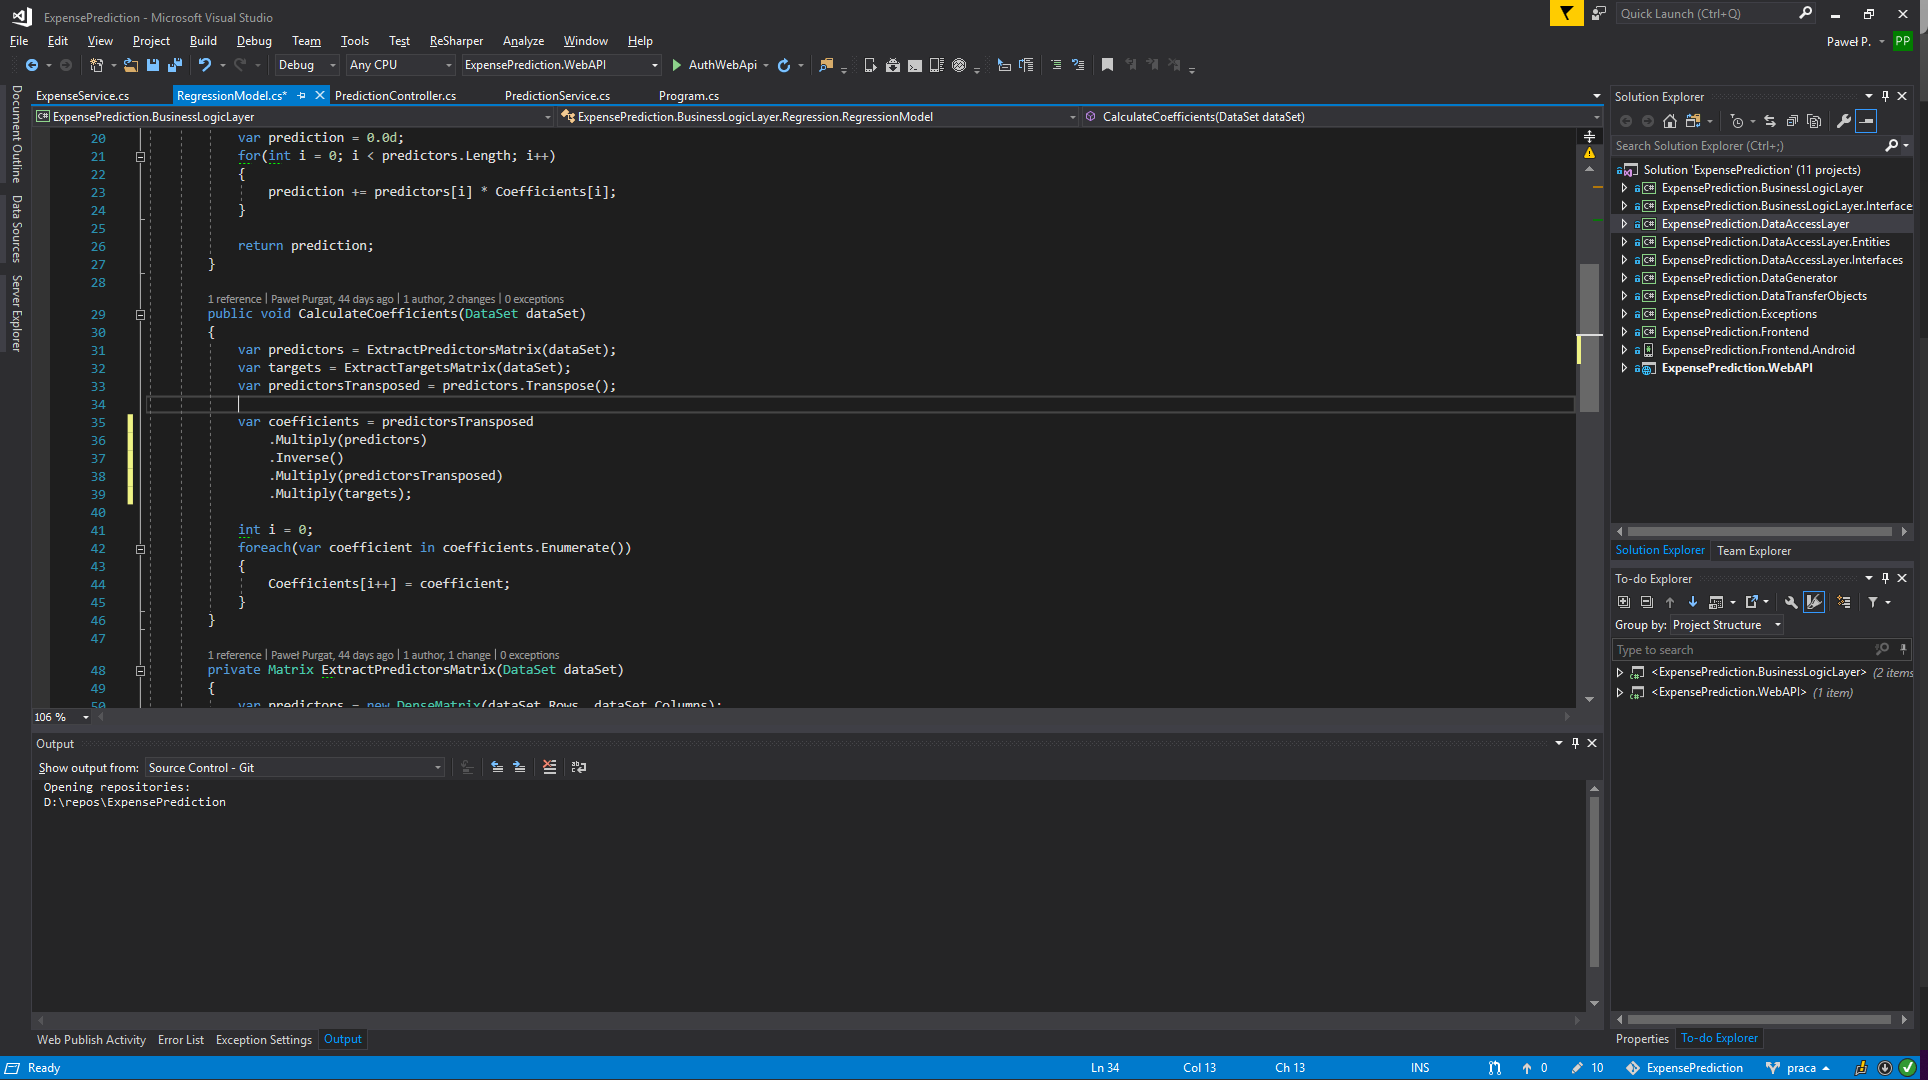
\includegraphics[width=6in]{img/aplikacje/vs_interfejs.png}
		\caption{Interfejs środowiska Microsoft Visual Studio}
		\label{vs_interfejs}
	\end{center}
\end{figure}

\textbf{ReSharper} (rys. \ref{resharper_interfejs}) jest narzędziem rozszerzającym środowisko Microsoft Visual Studio autorstwa JestBrains. Usprawnia ono proces wytwarzania oprogramowania poprzez automatyzację wielu procesów związanych z pisaniem wysokiej jakości kodu. Zapewnia ciągłą analizę kodu, co ułatwia wykrycie wielu błędów.\cite{resharper}
\begin{figure}[!ht]
	\begin{center}
		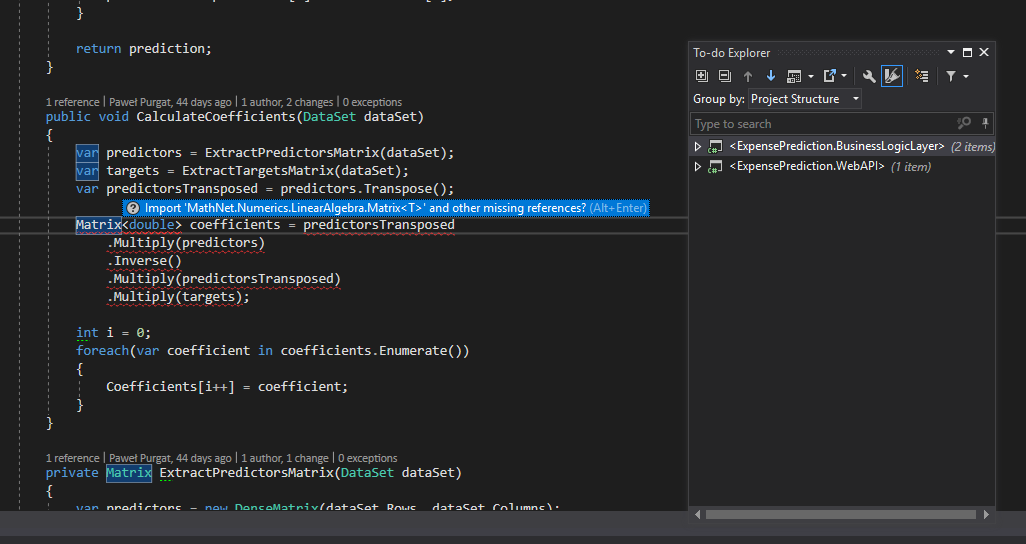
\includegraphics[width=6in]{img/aplikacje/resharper_interfejs.png}
		\caption{Przykładowe funkcjonalności rozszerzenia ReSharper}
		\label{resharper_interfejs}
	\end{center}
\end{figure}

\textbf{Postman} to aplikacja zapewniająca interfejs użytkownika służący do tworzenia i wysyłania zapytań do aplikacji internetowej. Zawiera ona kompleksowe narzędzia umożliwiające przegląd i analizę zapytań HTTP. \cite{postman}
\begin{figure}[!ht]
	\begin{center}
		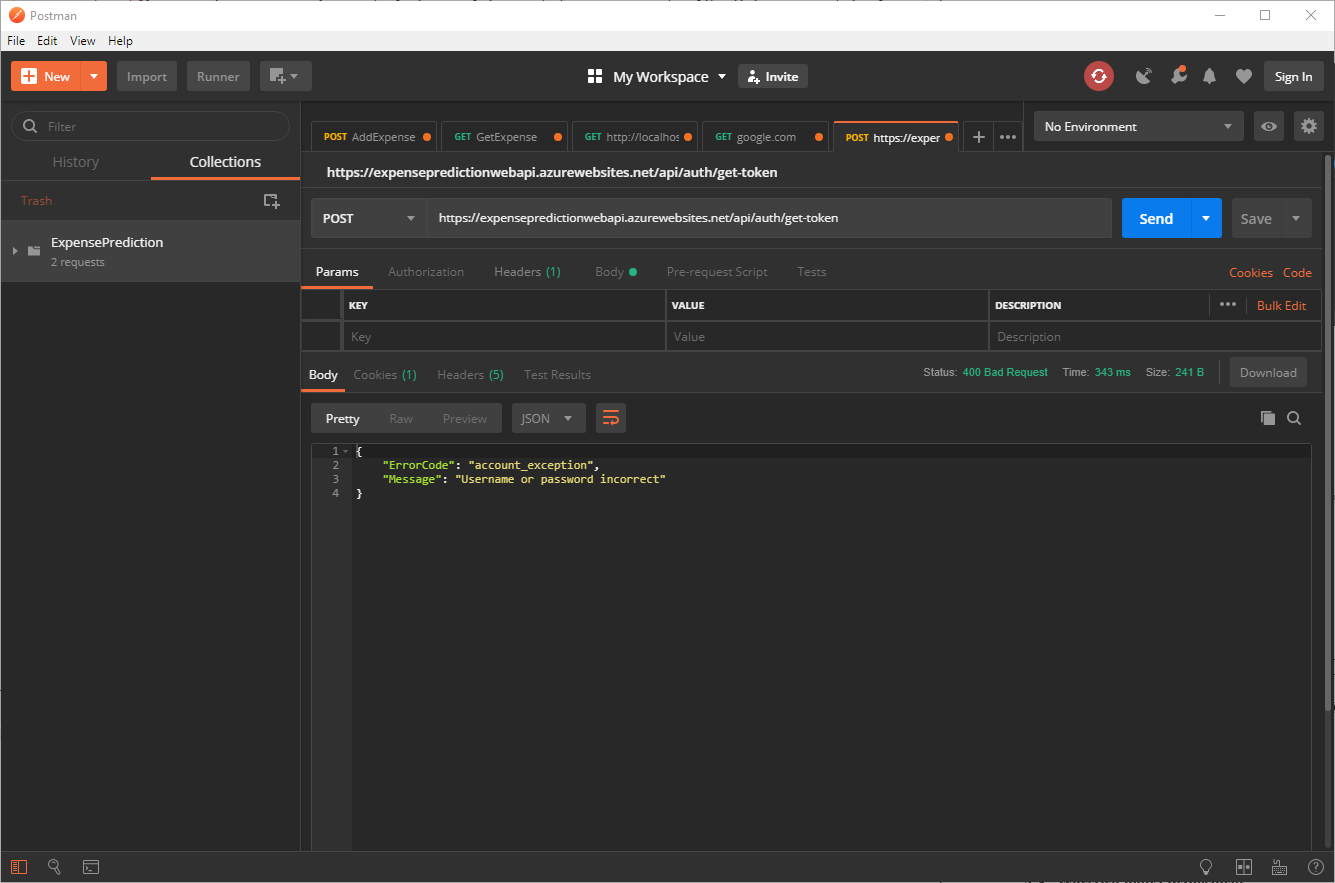
\includegraphics[width=6in]{img/aplikacje/postman_interfejs.png}
		\caption{Interfejs aplikacji Postman}
		\label{postman_interfejs}
	\end{center}
\end{figure}

\textbf{Swagger} (rys. \ref{swagger_interfejs}) jest narzędziem służącym do automatycznej dokumentacji kodu oraz zapewniającym konfigurowalny graficzny interfejs obrazujący stworzone API. Z poziomu wygenerowanego interfejsu możliwe jest proste konstruowanie zapytań zgodnych ze stworzoną aplikacją.\cite{swagger}
\begin{figure}[!ht]
	\begin{center}
		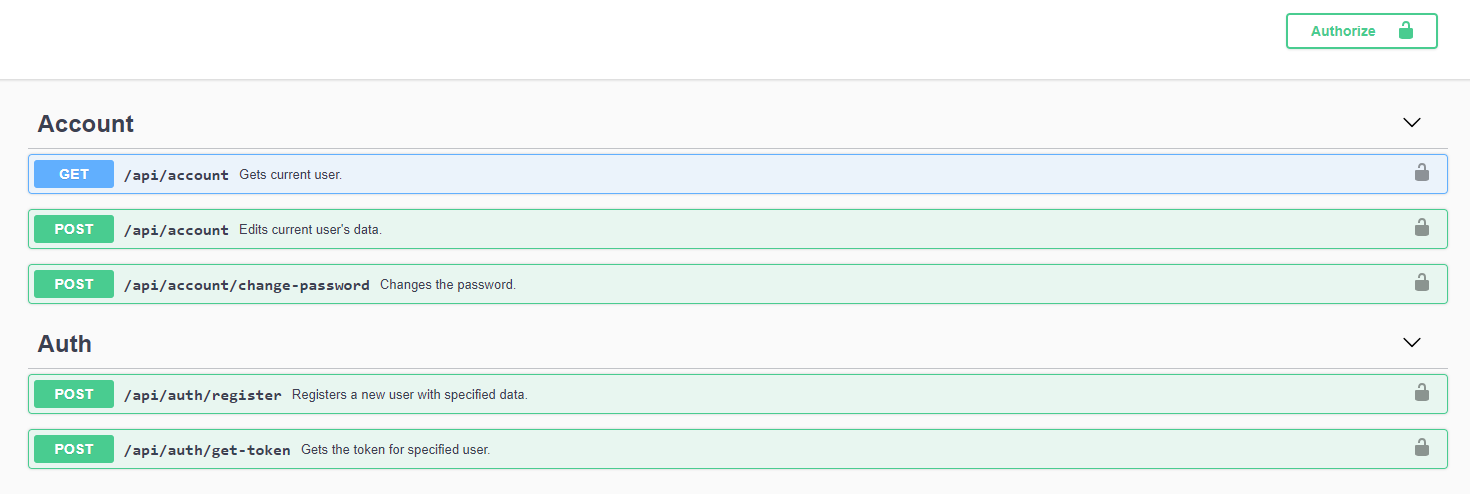
\includegraphics[width=6in]{img/aplikacje/swagger_interfejs.png}
		\caption{Interfejs wygenerowany przy użyciu narzędzia Swagger}
		\label{swagger_interfejs}
	\end{center}
\end{figure}

\textbf{REST (Representational State Transfer)} jest stylem projektowania systemów. Nie jest on standardem, lecz zbiorem reguł, takich jak bezstanowość, relacja klient - serwer oraz jednolity interfejs.\cite{rest}

\textbf{MVC (Model-View-Controller)} (rys. \ref{mvc}) to wzorzec projektowy polegający na podzieleniu projektu aplikacji na warstwy modelu danych, widoku, czyli interfejsu użytkownika oraz kontrolera, który reaguje na akcje wykonane przez użytkownika w warstwie widoku oraz odczytuje i modyfikuje dane z warstwy modelu.\cite{mvc}
\begin{figure}[!ht]
	\begin{center}
		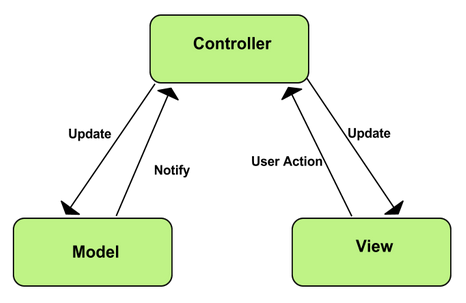
\includegraphics[width=5in]{img/diagram/mvc.png}
		\caption{Diagram przedstawiający wzorzec MVC (https://developer.chrome.com/static/images/mvc.png)}
		\label{mvc}
	\end{center}
\end{figure}

\textbf{Odwrócenie sterowania (ang. \textit{inversion of control})} jest techniką pozwalającą na skonstruowanie zależności w aplikacji zgodnie z kierunkiem abstrakcji, zamiast implementacji. W wielu aplikacjach zależności między klasami skonstruowane są na podstawie kolejności ich wykonania (rys. \ref{direct_dependency}).
\begin{figure}[!ht]
	\begin{center}
		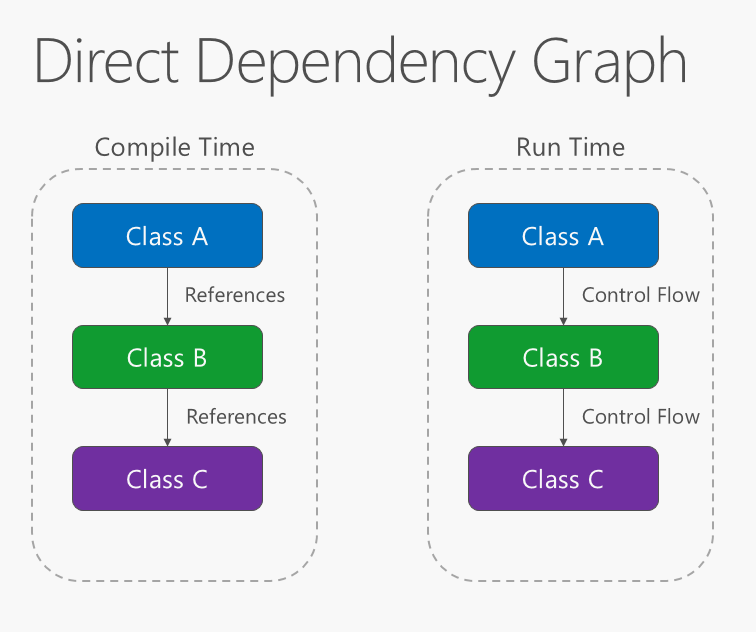
\includegraphics[width=6in]{img/diagram/direct_dependency.png}
		\caption{Diagram przedstawiający zależność bezpośrednią (https://docs.microsoft.com/en-us/dotnet/standard/ modern-web-apps-azure-architecture/media/image4-1.png)}
		\label{direct_dependency}
	\end{center}
\end{figure}
Odwrócenie sterowania polega na skonstruowaniu zależności w taki sposób, aby szczegółowa implementacja zależała od abstrakcyjnego komponentu (rys. \ref{inverted_dependency}).\cite{inversionofcontrol}

\begin{figure}[!ht]
	\begin{center}
		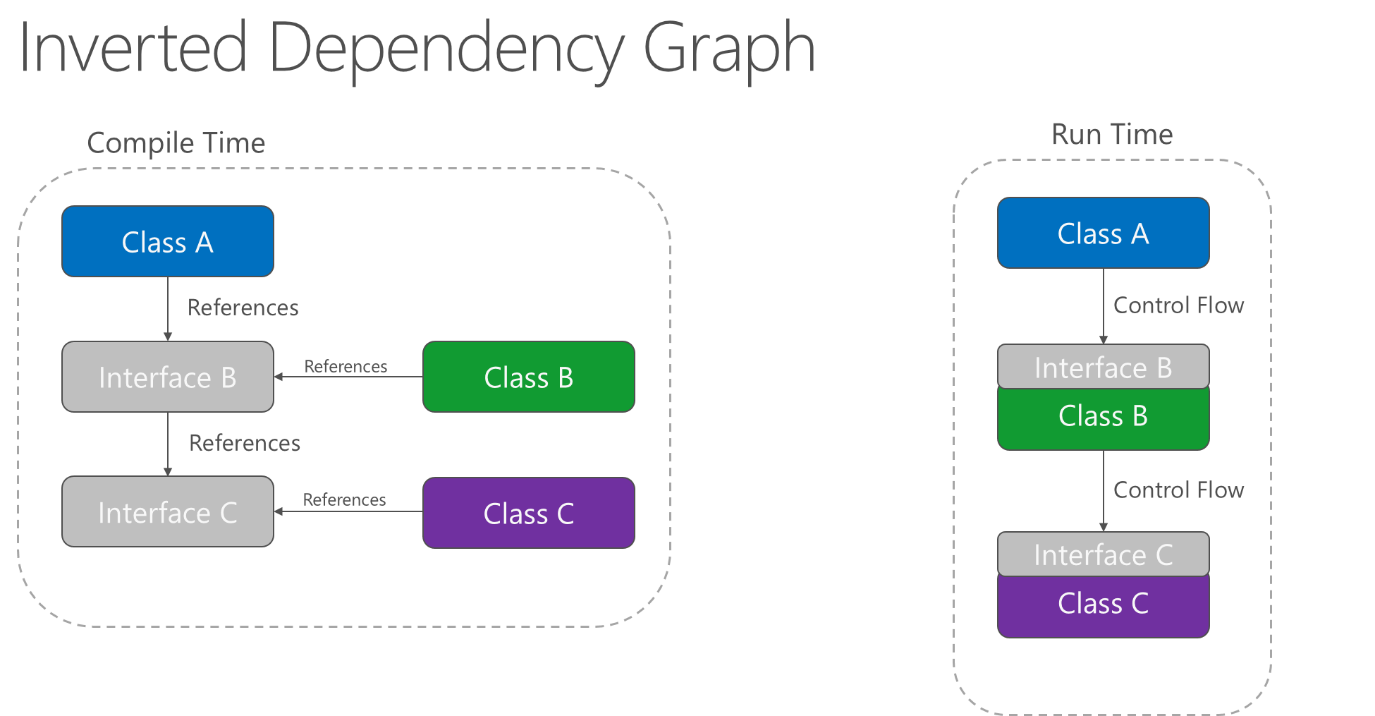
\includegraphics[width=6in]{img/diagram/inverted_dependency.png}
		\caption{Diagram przedstawiający zależność odwróconą (https://docs.microsoft.com/en-us/dotnet/standard/ modern-web-apps-azure-architecture/media/image4-2.png)}
		\label{inverted_dependency}
	\end{center}
\end{figure}
\textbf{Wstrzykiwanie zależności (ang. \textit{dependency injection})} jest wzorcem projektowym, który pozwala na osiągnięcie odwrócenia sterowania pomiędzy klasą a jej zależnościami poprzez przeniesienie odpowiedzialności za wybór implementacji abstrakcyjnego elementu na zewnętrzny kontener.\cite{dependencyinjection}

\textbf{Entity Framework Core} jest narzędziem realizującym mapowanie relacyjno-obiektowe (ang. \textit{object-relational mapping}) i oferującym możliwość odczytu i modyfikacji danych znajdujących się w bazie danych za pomocą klas reprezentujących encje w tej bazie.\cite{efcore}

\textbf{Language Integrated Query (LINQ)} to zbiór technologii których zadaniem jest zintegrowanie możliwości wykonywania zapytań na danych z językiem C\#. Zapewnia on jednolitą składnię tworzenia zapytań dla wielu źródeł danych, jak np. SQL, XML.\cite{linq}\\
Przyjmując, że kolekcja \textit{Users} i bazodanowa tabela o tej samej nazwie odnoszą się do tego samego zbioru danych, zapytanie LINQ (listing \ref{linqquery}) oraz zapytanie SQL (listing \ref{sqlquery}) zwróciłyby taki sam wynik.
\lstinputlisting[label={linqquery}, caption={Zapytanie LINQ.}, captionpos=b]{listing/query.cs}
\lstinputlisting[label={sqlquery}, caption={Zapytanie SQL.}, captionpos=b]{listing/query.sql}
\section{Biblioteki}
Dla środowiska .NET istnieje wiele zewnętrznych bibliotek. Dostępne są one poprzez system zarządzania pakietami NuGet. Narzędzie to pozwala na tworzenie oraz używanie bibliotek znajdujących się w repozytorium. W większości przypadków pakiety pobierane są z globalnego repozytorium dostępnego pod adresem \url{https://www.nuget.org}, jednakże istnieje możliwość tworzenia własnych repozytoriów i konfiguracji klienta NuGet do współpracy z nimi. W niniejszym podrozdziale opisane zostały jedynie biblioteki niewchodzące w skład frameworków Xamarin czy ASP .NET Core.

\textbf{AutoMapper} jest biblioteką umożliwiającą proste mapowanie jednego obiektu na drugi.\cite{automapper} Biblioteka ta pozwala na wzajemną konwersję dwóch typów poprzez przypisanie polom jednego obiektu wartości pól drugiego o takich samych nazwach. Taki zabieg jest konieczny np. przy mapowaniu obiektu klasy encyjnej na obiekt transferu danych (ang. \textit{data transfer object, DTO}).\\
Jeżeli pola obu typów mają takie same nazwy i nie wymagane jest żadne mapowanie między polami o różnych nazwach, definicja mapy sprowadza się do zdefiniowania typów, między jakimi ma powstać mapa (listing \ref{mapper_createmap}).
\begin{lstlisting}[label={mapper_createmap}, caption={Definiowanie mapowania między dwoma typami.}, captionpos=b]
mapperConfiguration.CreateMap<User, UserDto>();
mapperConfiguration.CreateMap<Expense, ExpenseDto>();
\end{lstlisting}
Przy tak zdefiniowanej mapie proces mapowania obiektów przebiega w sposób przedstawiony na listingu \ref{mapper_map}.
\begin{lstlisting}[label={mapper_map}, caption={Mapowanie jednego obiektu na drugi.}, captionpos=b]
User user = GetUser();
UserDto userDto = mapper.Map<UserDto>(user);
\end{lstlisting}

\textbf{MathNet.Numerics} jest biblioteką dostarczającą metody i algorytmy służące do wykonywania obliczeń i operacji numerycznych, m.in. algebry liniowej, modeli prawdopodobieństwa, interpolacji czy zagadnień optymalizacji.\cite{mathnetnumerics} W niniejszym projekcie biblioteka ta została wykorzystana w zakresie wykonywania operacji na macierzach (listing \ref{mathnetnumerics})
\begin{lstlisting}[label={mathnetnumerics}, caption={Operacje na macierzach przy użyciu biblioteki MathNet.Numerics.}, captionpos=b]
var predictors = ExtractPredictorsMatrix(dataSet);
var targets = ExtractTargetsMatrix(dataSet);
var predictorsTransposed = predictors.Transpose();

var coefficients = predictorsTransposed
.Multiply(predictors)
.Inverse()
.Multiply(predictorsTransposed)
.Multiply(targets);
\end{lstlisting}

\textbf{Newtonsoft.Json} to biblioteka służącą do obsługi danych w formacie JSON. Jest to wydajne narzędzie pozwalające między innymi na serializację i deserializację obiektów, stosowanie LINQ do ekstrakcji danych z formatu JSON oraz konwersję między JSON a XML.\cite{newtonsoft} Biblioteka ta jest najczęściej pobieranym pakietem z globalnego repozytorium NuGet.\cite{nugetstats}
%TODO: LIBRARIES, EF CORE